% Preamble
\documentclass[a4paper,doc,natbib]{apa6}

% Packages
\usepackage[english]{babel}
\usepackage[utf8x]{inputenc}
\usepackage{amsmath}
\usepackage{graphicx}
\usepackage{caption}
\usepackage{subcaption}
\usepackage{hyperref}
\usepackage{listings}
\usepackage{lipsum}

\title{Output correctness guarantees with LLM guardrails}
\shorttitle{Output correctness guarantees with LLM guardrails}
\author{Yasin G\"{u}l \and Arjan Broer}
\affiliation{Open University of the Netherlands}

\abstract{
    Large Language Models (LLMs) demonstrate impressive performance in a wide range of tasks, yet their outputs are not always correct or reliable.
    This introduces challenges in applications where factual or logical correctness is critical.
    This research investigates whether guardrails—mechanisms designed to constrain or verify model output—can provide guarantees for output correctness.
    Using a design research approach, we will iteratively develop and evaluate such guardrails, focusing on how correctness can be defined, implemented, and assessed.
    The study aims to identify what types of guarantees are feasible and what trade-offs are involved in enforcing them, with a particular focus on medical queries about medications.
}

% Document
\begin{document}

    \maketitle

\section{Introduction}
    % From the Research Methods workbook, page 241.
%
% In technical papers, the introduction presents the
% general background and the research questions. A detailed
% literature review is provided in the next section, called ‘Related
% work’. In the domain of psychology, which is more closely related
% to the study of how humans interact with AI, the introduction will
% contain the general background, literature review and research
% questions. There is some debate about whether to specify the
% research questions as actual questions, or to use phrases such as
% ‘This research will determine whether...’.

\subsection{Background}

Large Language Models (LLMs) are capable of generating coherent and contextually appropriate responses.
However, they occasionally produce hallucinations, factual inaccuracies, or unsafe advice.
This risk becomes particularly critical in medical contexts, where incorrect information can have serious consequences.
Recent research \citep{waldock2025curriculum} shows that LLMs can generate incorrect answers on medical prompts and students (or professionals) are required to valide the correctness of the output.
The study shows an accuracy rate of 50\% In this case the student acted as a human gaurdrail on the output of the LLM.

Examples include suggesting dangerous dosages, recommending inappropriate medications, or failing to warn against contraindications \citep{luo2024clinical}, \citep{schieszer2023large}.
For instance, providing a baby with an adult dose of ibuprofen, prescribing antibiotics for viral infections, or advising unsafe use of controlled substances are all examples where hallucinated outputs could cause harm.

A performance review of ChatGPT on the United States Medical Licensing Examination (USMLE) showed that the model performed at a level comparable to human physicians, but with a significant number of incorrect answers \citep{kung2023performance}.
This shows that the model can be expected to produce incorrect answers, even when it is capable of generating correct ones.

Guardrails have emerged as a strategy to mitigate these risks by constraining or verifying model outputs.
Techniques such as retrieval-augmented generation (RAG) and output moderation models have been proposed to systematically improve output reliability \citep{dong2024guardrails}.
Retrieval-augmented generation grounds answers in external, verified sources, reducing hallucinations, while moderator models can filter unsafe or incorrect content after generation \citep{inan2023llamaguard}.

In the medical domain, ensuring correct advice is even more crucial, particularly regarding medications.
Recent work shows that LLMs can contribute to reducing medication instruction errors when proper safeguards are in place \citep{pais2024medication}.

This proposal explores whether guardrails can be systematically designed and combined to guarantee correctness in LLM-generated answers for medication-related medical prompts.
We particularly investigate the effectiveness of retrieval-augmented generation and moderator models, individually and in combination, to prevent incorrect or unsafe medical advice.

\subsection{Research Questions}
This research explores the design and evaluation of guardrails that aim to ensure the correctness of outputs produced by LLMs for medication-related medical queries.
The central questions guiding this work are:

\begin{description}
    \item[RQ1.] Can a guardrail mechanism combining RAG and moderator models ensure 100\% correctness in LLM responses to medical prompts?
    \item[RQ2.] How can correctness be operationalized for medication-related queries (e.g., dosage, indications)?
    \item[RQ3.] What are the strengths and limitations of using RAG and moderator models in ensuring factual correctness in the medical domain?
\end{description}

\subsection{Null hypothesis}
The null hypothesis for this research is that the guardrail mechanisms (RAG, moderator model, and their combination)
do not significantly improve the correctness of LLM outputs compared to a baseline without guardrails.
In the below research methods section, a baseline condition is used to represent the LMM without guardrails.

    
\section{Methods}
    % From the Research Methods workbook, page 242.
%
%% This section explains how the research was performed.
% Sometimes it has a different name (e.g., ‘Experiments’), but still has
% the same purpose: to describe the methods. The section should
% allow another researcher to replicate the study (i.e., perform it
% again). This is different from obtaining the same findings). In
% psychology, this section has subsections describing participants,
% design, stimuli, procedure, and data analysis.

This project follows the design research methodology \citep{wieringa2014design}, consisting of iterative cycles of building, testing, and refining artifacts.
The artifact in this case is a guardrail mechanism for LLMs that constrains or validates generated output.

We test and compare four experimental conditions to evaluate the effectiveness of different guardrail approaches for ensuring correctness in medical prompts:

\begin{itemize}
    \item \textbf{Baseline:} No guardrails applied.
    \item \textbf{RAG-only:} Responses are grounded in external verified medical sources using retrieval-augmented generation \citep{dong2024guardrails}.
    \item \textbf{Moderator-only:} A second AI model evaluates the generated output and flags or blocks incorrect or unsafe content \citep{inan2023llamaguard}.
    \item \textbf{Combined:} Both RAG and moderator-AI are applied sequentially, first applying RAG grounding, followed by moderator verification.
\end{itemize}

The evaluation focuses on whether the guardrail meets defined correctness criteria in realistic scenarios and what design choices contribute to its effectiveness.

\subsection{Baseline setup}
In the baseline setup (\autoref{fig:baselineSetup}) we use a large language model (LLM) to generate responses to medical prompts without any guardrails.
The model used is the Google Gemini 2.0 flash model, which is a large language model trained on a wide range of data, including medical texts \citep{saab2024capabilities}.
The medical questions are directly used as prompt for the LLM.
Later iterations of the project proved that the medical question needed to be extended with additional patient information.
The information was primarily needed for manual review by an expert user as the medical context of the patient is important to validate if the recipe is correct.
Together with the prompt the LLM is provided with a system instruction that specifies the task and expected output format.
As the medical question if formulated in Dutch, the system instruction is also in Dutch.
\begin{verbatim}
    Je bent een medisch expert. Beantwoord de medische vraag met
    een recept volgens het volgende template:
    'Rp. [Medicijnaam] [Sterkte] [Vorm]\ndtd. No. [Aantal]\n S. [Instructie]'.
    Neem relevante informatie over de patiënt in acht, zoals leeftijd en
    eventuele allergieën.
    Geef de formele medicijnnaam in het JSON-veld 'medicijn'.
    Benoem de categorie van het medicijn in het JSON-veld 'categorie'.
    Geef bij de instructie ook de duur van de behandeling aan.
    Herhaal de medische vraag in het JSON-veld 'medische_vraag'.
    Voeg de patiëntinformatie toe in het JSON-veld 'patientinformatie'.
\end{verbatim}

\begin{figure}[H]
    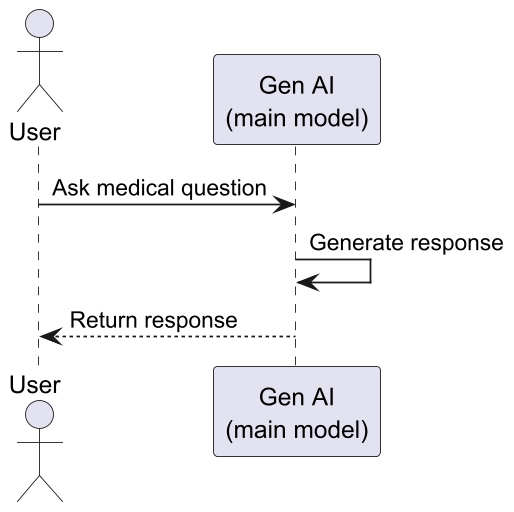
\includegraphics[width=0.5\textwidth]{figures/baselineSetupSequenceDiagram.png}
    \captionof{figure}{Baseline setup for generating medical recipes without guardrails.}
    \label{fig:baselineSetup}
\end{figure}

\subsection{RAG-only setup}

In the RAG-only setup (\autoref{fig:ragSetup}), we use a large language model (LLM) to generate responses to medical prompts and check the response using retrieval-augmented generation (RAG).
The RAG component retrieves relevant information about the medication from apotheek.nl and uses that information to validate the generated output.
The output is validated for correctness of medicine, dosage, shape, frequency and instruction taking the context of the patient information into consideration.
When the output is not correct the response will be reported as false.
This allows the system to take corrective actions when the response is incorrect.

\begin{figure}[H]
    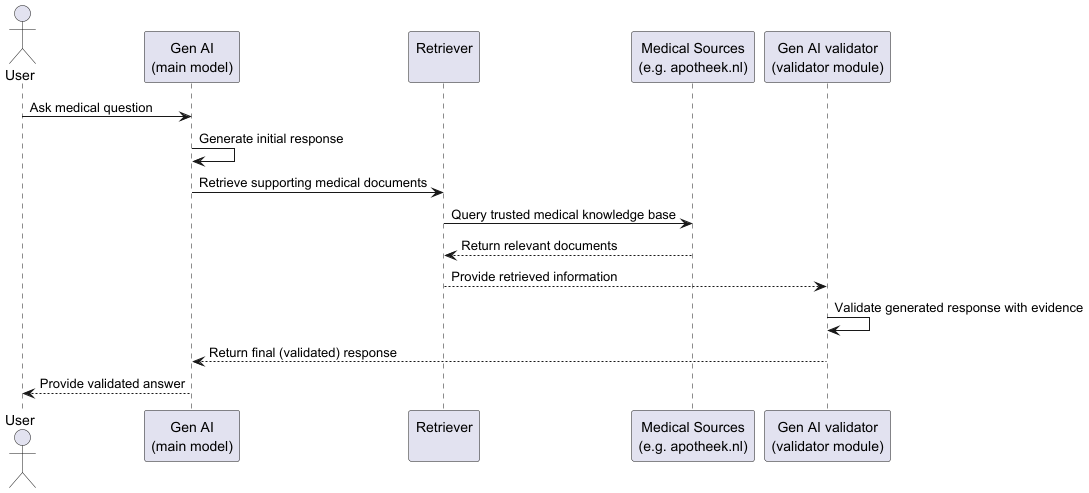
\includegraphics[width=0.5\textwidth]{figures/RAGSetupSequenceDiagram.png}
    \captionof{figure}{RAG-only setup for generating medical recipes with retrieval-augmented generation.}
    \label{fig:ragSetup}
\end{figure}

\subsection{Moderator-only setup}

In the moderator-only setup (\autoref{fig:moderatorSetup}), we use a large language model (LLM) to generate responses to medical prompts and check the response with a moderator LLM model.
The moderator model evaluates the generated output and flags or blocks incorrect or unsafe content.
The same LLM model is used for both the generation and moderation tasks, but with different system instructions.

\begin{figure}[H]
    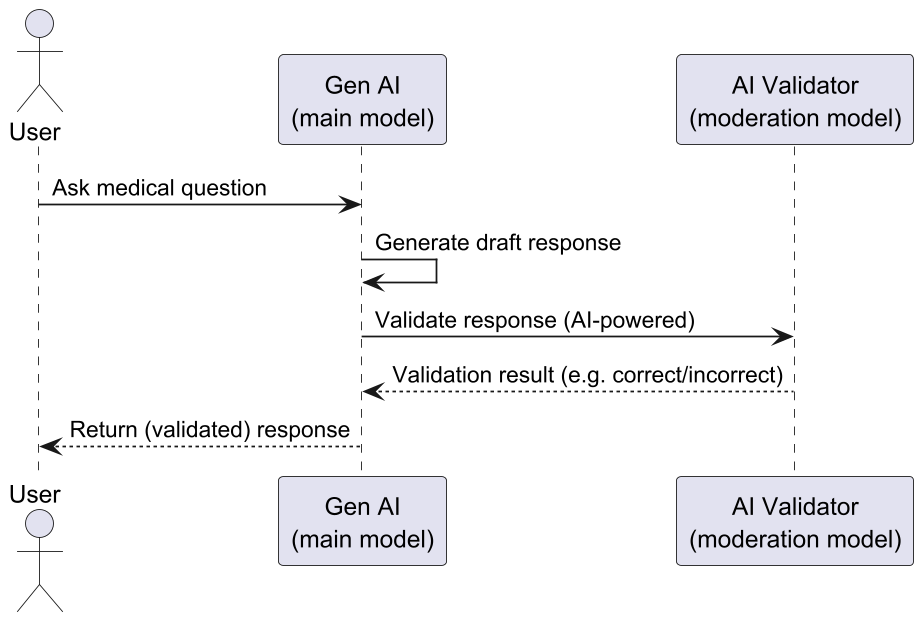
\includegraphics[width=0.5\textwidth]{figures/moderatorSetupSequenceDiagram.png}
    \captionof{figure}{Moderator-only setup for generating medical recipes with a moderator model.}
    \label{fig:moderatorSetup}
\end{figure}

\subsection{Combined setup}

In the combined setup (\autoref{fig:combinedSetup}), we use a large language model (LLM) to generate responses to medical prompts and check the response with both retrieval-augmented generation (RAG) and a moderator model.
The RAG component retrieves relevant information about the medication from apotheek.nl and uses that information to validate the generated output.
The moderator model evaluates the generated output and flags or blocks incorrect or unsafe content.
The recipe is considered correct when it is both grounded in the retrieved information and passes the moderation check.

\begin{figure}[H]
    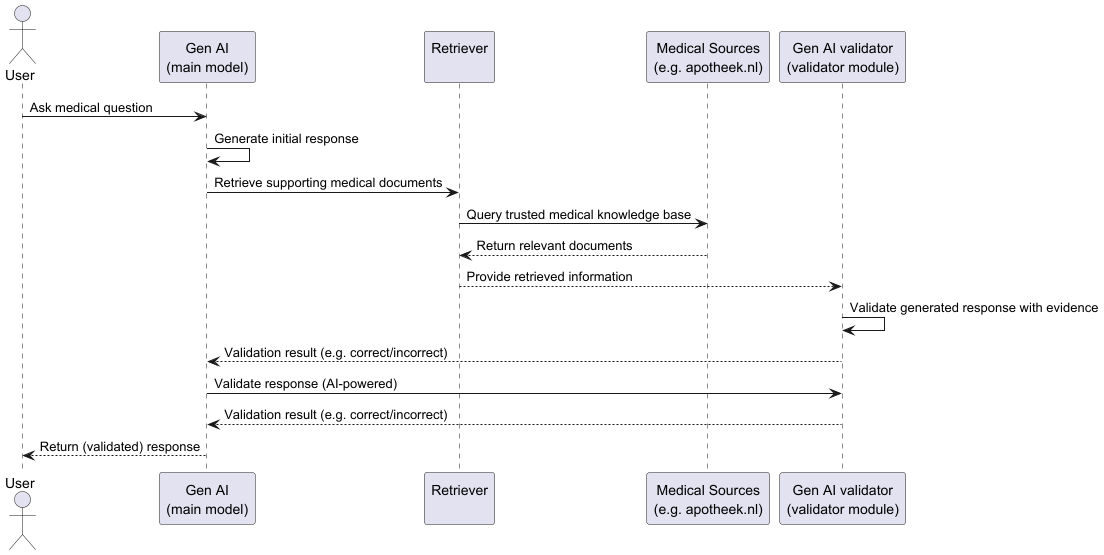
\includegraphics[width=0.5\textwidth]{figures/combinedSetupSequenceDiagram.png}
    \captionof{figure}{Combined setup for generating medical recipes with retrieval-augmented generation and a moderator model.}
    \label{fig:combinedSetup}
\end{figure}

\subsection{Apparatus}

The LLM used for the baseline, RAG-only, moderator-only, and combined setups is the Google Gemini 2.0 flash model.
No changes have been made to the model parameters like temperature or top-p sampling, as the model is already optimized for generating high-quality responses.
To be able to process the entire dataset efficiently, the medical questions and recipes are processed in the baseline setup as one batch of 200 questions.
For running the guardrail mechanisms, the model is called in a loop for each baseline answer.
This setup deviates from the intended guardrail setup, but makes data analysis easier and more efficient.
When the initial prompt to the model would generate different answers the performance of the guardrail mechanisms would be harder to compare.
Feeding the same baseline answers to all guardrail mechanisms allows for a fair comparison of the performance of the different guardrail mechanisms.

\subsection{Stimuli}

To evaluate the guardrails, we use a fixed set of prompts that represent medical questions including patient information.
These tasks represent real-world LLM use cases with identifiable correctness constraints \citep{pais2024medication}.
The responses are formatted as formal medical recipes following the Dutch guidelines for medication prescriptions \citep{farmacotherapeutischkompas}.
\begin{verbatim}
        Rp.   [Medicijnnaam] [Sterkte] [Vorm]
          dtd. No. [Aantal]
          S. [Instructie]
\end{verbatim}

The RAG guardrail first finds the medication information on apotheek.nl using a Google search.
The relevant information is extracted from the retrieved web page and fed to the LLM as part of the prompt.
The moderator guardrail uses a similar system instruction as the RAG guardrail, but will not use the retrieved information.

\subsection{Dataset}

The dataset consists of a set of 200 medical questions and relevant patient information including age, gender and symptoms.
The medical questions and patient information will be used as prompt input for the baseline setup to generate answers as recipes.
The recipes will be used by the guardrails to evaluate the correctness of the generated output.
Because patient information is subject to privacy regulations, the dataset is completely synthetic and has been generated by the researchers.
To make sure the dataset is representative of real-world medical questions all questions and patient information has been reviewed by a medical expert.

\subsection{Design}

Each medical question and patient information is used for the baseline setup to generate the initial set of recipes.
The same set of recipes is used for manual expert review, RAG-only setup, moderator-only setup, and combined setup.
Performance is evaluated by comparing the guardrail setups to the manual review.
The manual review by the medical expert is assumed to be correct.
The same dataset of recipes is used for all guardrail setups, ensuring a fair comparison.

Both the RAG setup and the moderator setup use a similar system instruction to generate the recipes.
The only difference is that the RAG system instruction tells the LLM to use the text in 'Details' to validate the recipe.
This ensures that both guardrail mechanisms evaluate the recipes on the same criteria.

moderator system instruction:
\begin{verbatim}
Beoordeel het recept op basis van de volgende criteria:
1. Bevat het medicijn een geldige naam, sterkte, vorm, aantal doses en instructies?
2. Is de indicatie relevant voor de medische vraag en gegeven patient informatie?
3. Is het recept de juiste keuze voor de eerste behandeling van de medische vraag?
4. Geef een beoordeling van het recept als correct = True|False.
\end{verbatim}


RAG system instruction:
\begin{verbatim}
Beoordeel met de tekst in 'Details' het recept op basis van de volgende criteria:
1. Bevat het medicijn een geldige naam, sterkte, vorm, aantal doses en instructies?
2. Is de indicatie relevant voor de medische vraag en de gegeven patient informatie?
3. Is het recept de juiste keuze voor de eerste behandeling van de medische vraag?
4. Geef een beoordeling van het recept als correct = True|False.
\end{verbatim}

\subsection{Procedure}

The research is conducted in the following steps:
\begin{enumerate}
    \item Create the dataset of 200 medical questions and patient information.
    \item Run the baseline setup to generate recipes for all medical questions.
    \item Conduct a manual expert review of the generated recipes to establish correctness criteria.
    \item For each recipe perform a correctness check with the RAG-only setup, the moderator-only setup, and the combined setup.
    \item Evaluate the performance of each guardrail setup against the manual expert review on precision and recall.
    \item Analyze failures, compare effectiveness, and refine guardrail designs.
\end{enumerate}

These steps have been repeated in an iterative design cycle, where each iteration refines the guardrail mechanisms based on the results of the previous iteration.
We avoided regeneration of the recipes from the baseline set to reduce the workload on the medical expert.
As a consequence the iterations were not fully independent, but the results of the previous iteration were used to improve the next iteration.

\subsection{Data analysis}

Each guardrail setup (Baseline, RAG-only, Moderator-only, Combined) is evaluated using the following metrics:

\begin{itemize}
    \item \textbf{Error rate:} Percentage of incorrect or unsafe answers.
    \item \textbf{Precision/Recall:} For detecting unsafe or medically incorrect outputs.
    \item \textbf{False positives / negatives:} Analysis of over- or under-blocking.
\end{itemize}

This comparison allows us to determine whether a specific approach—or their combination—can achieve 100\% correctness or significantly reduce critical errors.

\subsection{Code Repository}
The code for this research is available on GitHub at \url{https://github.com/abroer/IM1312}


\section{Results}
    \subsection{Overall Model Performance}

We tested three different approaches: RAG, Moderator, and Combined, on a set of 200 medication-related questions. The outcomes were compared to a manual review, which acted as our gold standard for correctness. According to this review, 140 of the answers were considered correct and 60 were incorrect.

Looking at Figure~\ref{fig:prediction_performance_bar}, the differences between the models quickly become clear. Moderator picks up the most correct answers, with 133 true positives, and misses only 7 false negatives. However, it also produces the most false positives at 50, which means it can be too generous in what it accepts as correct. Its true negatives are low, only 9, showing it is not strict in filtering out wrong answers.

RAG finds 109 true positives and 28 true negatives. Both false positives and false negatives stand at 31, which suggests this approach sits right in the middle. RAG does not lean toward one type of error and can be seen as a neutral or balanced option.

The Combined approach is the most careful. It only accepts 104 correct answers and misses 36, so it tends to overlook good answers. On the upside, it produces the fewest false positives at 28 and the highest number of true negatives at 31. This tells us that Combined is the strictest in its standards.

\begin{figure}[ht]
  \centering
  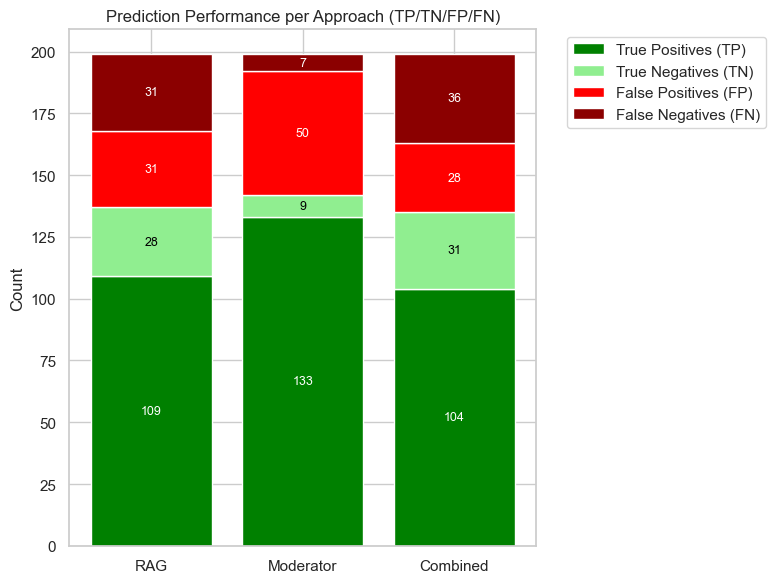
\includegraphics[width=0.95\linewidth]{figures/prediction_performance_per_approach.png}
  \caption{Prediction Performance per Approach, showing true positives, true negatives, false positives, and false negatives for RAG, Moderator, and Combined.}
  \label{fig:prediction_performance_bar}
\end{figure}

\subsection{Performance Metrics and Trade-offs}

Figure~\ref{fig:model_performance_comparison_per_metric} shows the key performance numbers for each model: precision, recall, F1 score, and accuracy. Moderator scores highest on recall at 95.0 percent, so it almost never misses a correct answer. The trade-off is that its precision drops to 72.7 percent, as it tends to let more incorrect answers through. Combined flips this pattern and is most careful in what it approves, with a precision of 78.8 percent, but its recall drops to 74.3 percent, so it lets more good answers slip by. RAG sits right in the middle, with precision and recall both at 77.9 percent.

When we look at F1 score and accuracy, Moderator comes out on top, but not by much. Its F1 score is 82.4 percent, and accuracy is 71.4 percent. RAG and Combined follow closely behind. This mix of strengths and weaknesses in each model reflects the real-world trade-offs you face when choosing a guardrail approach.

\begin{figure}[ht]
  \centering
  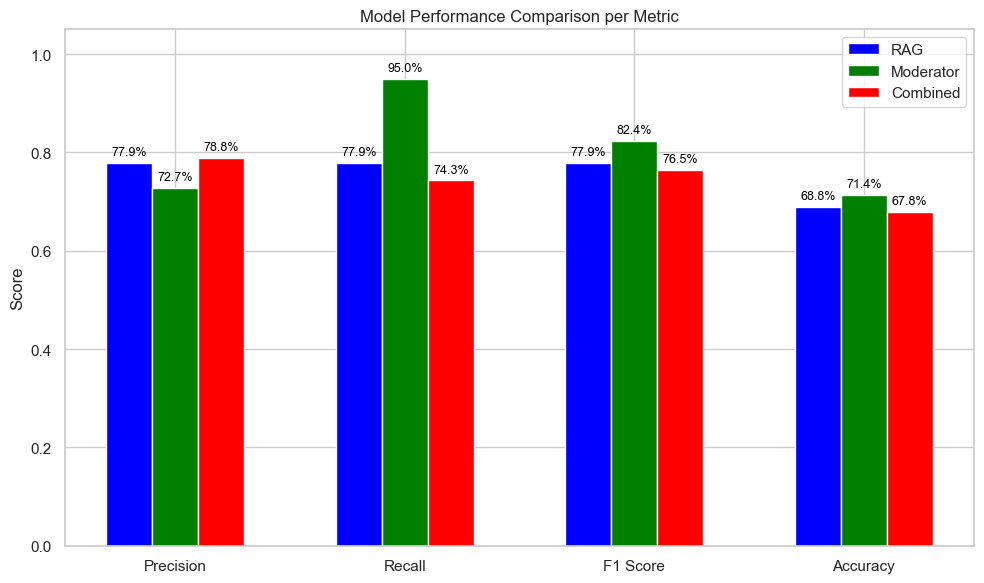
\includegraphics[width=0.95\linewidth]{figures/model_performance comparison_per_metric.png}
  \caption{Model Performance Comparison per Metric: precision, recall, F1 score, and accuracy for each model.}
  \label{fig:model_performance_comparison_per_metric}
\end{figure}

\subsection{Results on individual Questions}
To give a clearer picture of how each model performs, we looked at the results for individual questions.
The bar charts in \autoref{fig:dna-results} show which answers were positive (green) and which were negative (red) for each model.
The expectation is that when both RAG-only and Moderator-only are positive, the Combined model should also be positive.
However, this is not always the case. For example, in question 10, RAG-only and Moderator-only are both positive, but Combined is negative.
The number of occurrences that this happens is low (12), but it does show some instability of the behavior of the models.

Something similar happens in question 79, where either RAG-only is negative, but Combined is positive.
The expectation is that if RAG-only is negative, Combined should also be negative, but this is not the case.
The number of occurrences that this happens is very low (4), but it again shows that the models are not always consistent.

The exact same code, prompt and system instruction has been used for RAG and Moderator in the Combined model.
So, the expectation is that the behavior in RAG-only/Moderator-only should be the same as in Combined.
The inconsistencies must be found in other external factors which is further explored in the discussion section.

\begin{figure}[H]
    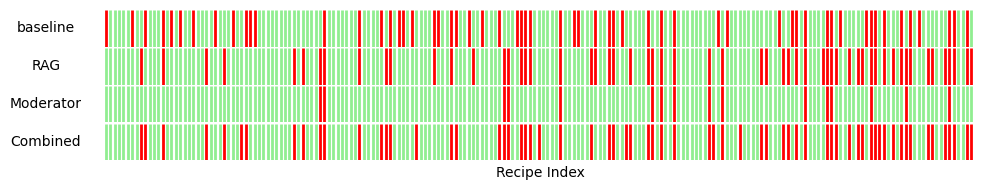
\includegraphics[width=1\linewidth]{figures/dna-results.png}
    \caption{Results on individual questions for each model, positive (green) and negative (red) answers.}
    \label{fig:dna-results}
\end{figure}

\subsection{Can Perfect Correctness Be Achieved?}

One of the main questions in this research was whether combining RAG and Moderator could guarantee perfect correctness. The short answer is no. Even the combined approach falls short. It gives 104 true positives and 36 false negatives. While it does cut down on false positives, it still misses a fair number of correct answers. No model in this study produced perfect results.

\subsection{How Was Correctness Defined?}

Throughout this project, correctness was defined using a strict set of criteria. An answer was only considered correct if it matched the manual reviewer's judgment on both the medical content and whether the medication, dosage, and indication were appropriate. Every performance metric reported here uses this definition.

\subsection{Summary}

To sum up, each model has its own personality. Moderator hardly misses any correct answers but is not picky enough, letting through a lot of false positives. Combined is picky and almost to a fault, which means it avoids false positives but also overlooks more good answers. RAG sits comfortably in the middle, with no big risks either way. None of the models manages to be perfect, so the best choice depends on what kind of error matters most for your application. Figures~\ref{fig:prediction_performance_bar} and~\ref{fig:model_performance_comparison_per_metric} offer a visual summary of these findings.



\section{Discussion}
    % From the Research Methods workbook, page 242.
%
% This section usually starts with a one- or two-line
% summary of the aim of the study and the main result or results. It
% compares the findings against the literature, and explains why
% some differences (if any) may have been found. This section
% sometimes contains the limitations of the study and suggestions for
% future work. It often ends with a conclusion.

This study explores whether guardrails, specifically retrieval-augmented generation (RAG), moderator models, and their combination, can ensure correctness in LLM-generated responses to medication-related medical prompts.
While all three guardrail setups improved upon the baseline, none achieved perfect correctness, highlighting both the promise and limitations of current guardrail strategies.

\subsection{Performance findings and trade-offs}
The results reveal a clear trade-off between precision and recall across the different guardrail mechanisms:

\begin{itemize}
\item Moderator-only achieved the highest recall (95.0\%), indicating it was most effective at identifying correct answers.
    However, it also had the highest false positive rate, suggesting a tendency to over-approve potentially unsafe or incorrect outputs.
\item RAG-only offered a more balanced performance, with moderate precision and recall (both 77.9\%), but still struggled with both false positives and false negatives.
\item Combined guardrails yielded the highest precision (78.8\%), meaning it was most conservative in approving only correct answers.
    However, this came at the cost of recall (74.3\%), as it missed a significant number of correct responses.
\end{itemize}
These findings suggest that while combining RAG and moderator models can reduce the risk of approving incorrect outputs, it may also lead to under-approving correct ones—an important consideration in clinical contexts where both false positives and false negatives carry risks.
This performance still includes a significant number of false positives and false negatives, up to the level where it is not safe to use the LLM-generated responses in a clinical setting without further human review.

\subsection{Inconsistent Model Behavior}
The confusion matrices and individual question breakdowns reveal inconsistencies in model behavior.
Notably, there were 12 cases where both RAG and Moderator approved an answer, but the Combined model did not.
This suggests that the sequential application of guardrails may yield unexpected differences in outcomes, making the model unreliable in certain scenarios.

Conversely, in 4 cases, the Combined model approved answers that RAG alone had rejected.
Again this highlights unexpected behvaior in the models, where same prompts can lead to different outcomes.

Causes of the inconsistencies may include:
\begin{itemize}
    \item Temperature settings, which influence the randomness of the model's responses.
    \item Top-p sampling, which controls the diversity of the generated text.
\end{itemize}
Further research is needed to understand how these parameters affect model behavior and output stability.

\subsection{Correctness Criteria and Operationalization}
Correctness was operationalized based on expert-reviewed criteria: appropriate medication, dosage, and indication tailored to patient context.
This strict definition ensured clinical relevance but may have penalized otherwise reasonable alternatives.
Future work could explore graded correctness or confidence scoring to better reflect real-world clinical decision-making, where multiple valid options may exist.
The introduction of reasoning and cofidence scoring has been explored in \autoref{kang2024r}.
A similar approach could be applied to the guardrail approaches in this study to better reflect the clinical decision-making process.

\subsection{Input Quality and Model Limitations}
The quality of the input prompts significantly influenced model performance.
During the manual review phase the expert reviewer indentified that some medical questions were incomplete or relevant patient information was missing.
This highlights the importance of high-quality, well-structured prompts in eliciting accurate model responses.
Further improvement of the performannce cna be achieved by introducing input guardrails to ensure that the input is up to a level where reasonalble answers can be expected.
For interactive applications the input guardrails can be used to guide the user to provide the necessary information.
This will make sure that the input passes only when a certain level of input quality confidence is reached.
An implementation that mimics the interaction of a medical professional with a patient is described in \autoref{hsu2025medplan}.

\subsection*{Conclusion}
This research demonstrates that guardrails can significantly improve the correctness of LLM outputs in medical contexts, but no single researched approach guarantees perfection.
The choice of guardrail depends on the desired balance between safety (precision) and inclusivity (recall).
A combined approach offers the most conservative filtering, but may miss valid answers.
Future research should focus on refining guardrail logic, exploring input validation, and testing across diverse guardrail models to build more trustworthy AI systems for healthcare.


\bibliography{literature}


\end{document}